% Preamble
\documentclass[11pt]{article}
\usepackage[margin=1in]{geometry}
\usepackage{amsmath}
\usepackage{amsfonts}
\usepackage{amssymb}
\usepackage{graphicx}
\usepackage{subcaption}
\usepackage{xcolor}
\usepackage{enumerate}
\usepackage{hyperref}
\usepackage{url}
\usepackage{fancyhdr}

% Header setup
\pagestyle{fancy}
\fancyhf{}
\fancyhead[L]{MIT Open Learning - Universal AI}
\fancyhead[R]{Transportation}
\renewcommand{\headrulewidth}{2pt}
\renewcommand{\footrulewidth}{0pt}

% Document
\title{Homework 1: Introduction to AI for Transportation}
\author{Riccardo Fiorista | \href{mailto:riccardo-uai@mit.edu}{riccardo-uai@mit.edu}}
\date{August, 2025}

\begin{document}
\maketitle
\thispagestyle{fancy}

\section*{Lecture Summary}

Professor Zhao's lecture introduced AI for Transportation through four key sections: defining success vs. progress, understanding transportation systems and data, real-world grounded AI applications, and generative AI opportunities.

The central challenge: technological progress doesn't automatically equal success. Beijing's transformation from sustainable bicycles to car-dominated congestion exemplifies this paradox. Despite technological advances, transportation faces 42,915 annual US traffic fatalities (vs. 120 airline deaths in 2023), 28\% of greenhouse gas emissions, and persistent accessibility issues.

The course bridges \textbf{behavioral thinking} (travel as social, emotional, perceptual) with \textbf{computational thinking} (data, algorithms, AI) to create truly successful transportation systems. These exercises focus on the subjective, value-driven aspects of applying AI responsibly in your chosen domain.

\section*{Exercise 1: Defining Success}

\begin{center}
\fcolorbox{gray}{lightgray}{%
\begin{minipage}{0.6\textwidth}
\centering
\vspace{3mm}
\Large Define success \& the future for your field/industry/community \\
in the light of: Data, AI, and Behavior
\vspace{3mm}
\end{minipage}%
}
\end{center}

Prof. Zhao showed how progress doesn't equal success using Beijing's shift from sustainable transport to car-dominated congestion. Success requires defining metrics before introducing new technologies.

Choose a field you know well and analyze three aspects: \textit{current state}, \textit{desired future}, and what makes the transition a \textit{success}. Move beyond economic benefits to consider data, AI, and behavioral dimensions across safety, sustainability, equity, and efficiency.

\subsection*{Instructions:}
\begin{enumerate}[(a)]
\item \textbf{Choose your domain:} Select a field, industry, or community where you have substantial knowledge or experience.

\item \textbf{Current State Analysis:} Describe the current challenges and limitations in your chosen domain. Consider:
\begin{itemize}
\item What are the main problems that parallel transportation's issues (safety, sustainability, equity, efficiency)?
\item How is data currently collected and used?
\item What behavioral patterns drive current outcomes?
\end{itemize}

\item \textbf{Future Vision:} Articulate your vision for the future of this domain. Consider:
\begin{itemize}
\item What would a truly successful transformation look like?
\item How might AI's five core functions (represent, predict, explain, control, create) improve outcomes?
\item What behavioral changes would be necessary?
\end{itemize}

\item \textbf{Success Metrics:} Define concrete, multi-dimensional measures of success that go beyond traditional economic indicators. Consider:
\begin{itemize}
\item How will you measure progress toward your vision?
\item What metrics capture the human, social, and environmental dimensions?
\item How can these metrics prevent the "Beijing paradox" of technological progress without true improvement?
\end{itemize}
\end{enumerate}

\noindent\textbf{Goal:} Reflect on the three components above.

\section*{Exercise 2: Systems Thinking and Analytics Framework}

\begin{center}
\fcolorbox{gray}{lightgray}{%
\begin{minipage}{0.6\textwidth}
\centering
\vspace{3mm}
\Large Create a similar analytics framework diagram \\
for your chosen field/industry/community
\vspace{3mm}
\end{minipage}%
}
\end{center}

\begin{figure}[h]
\centering
\begin{subfigure}{0.48\textwidth}
\centering
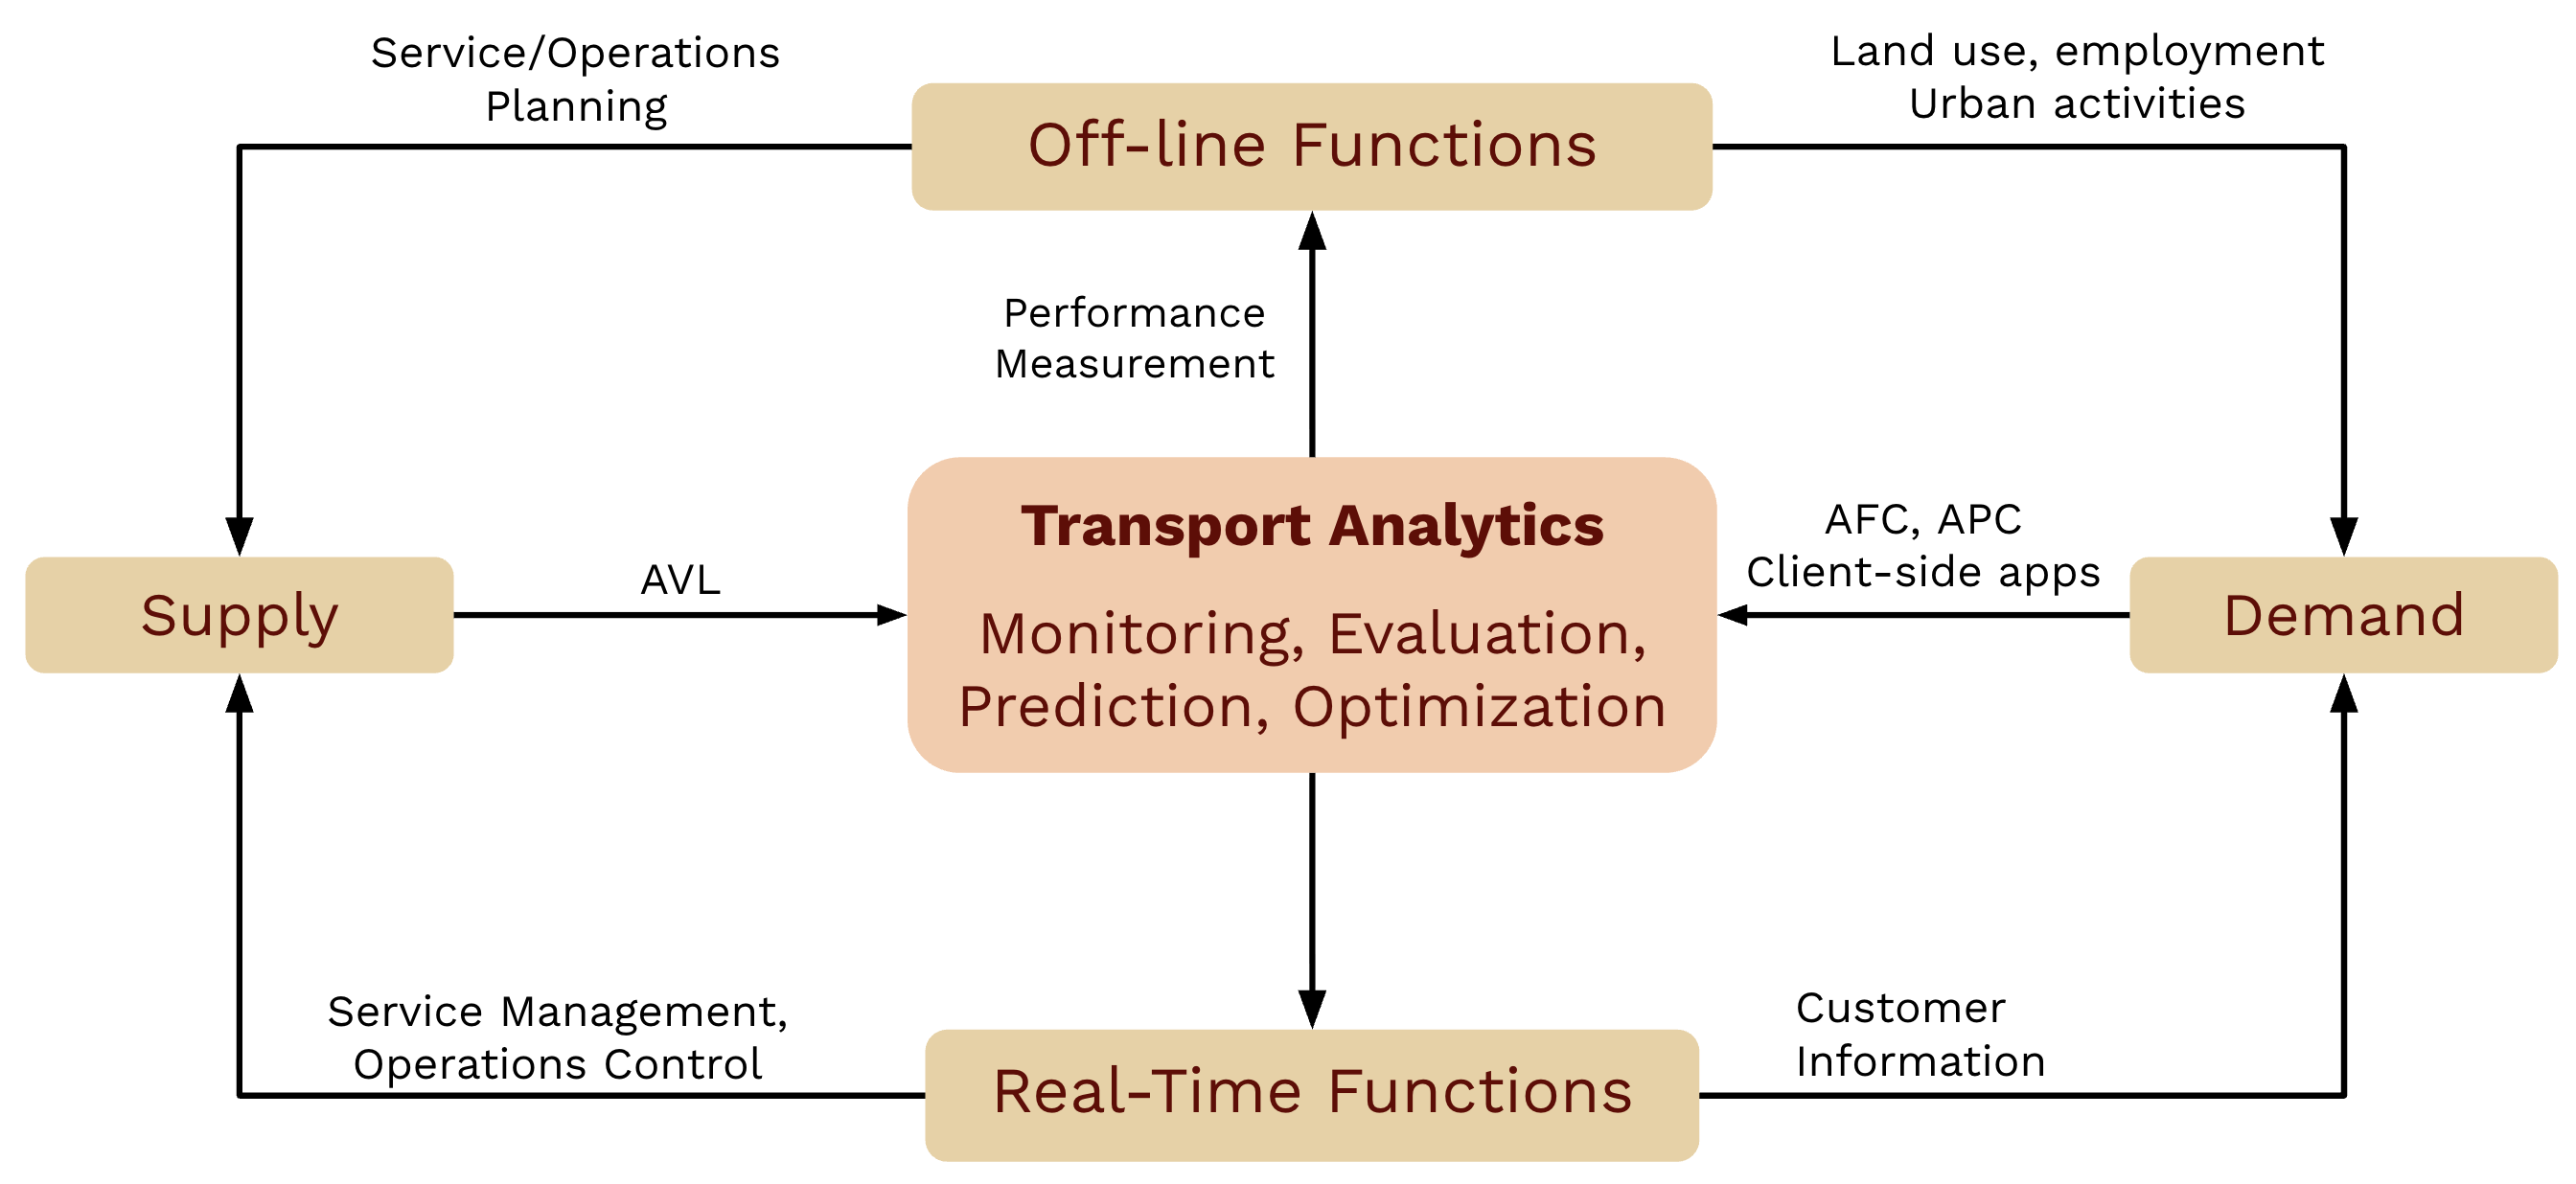
\includegraphics[width=\textwidth]{transport_analytics_graph.png}
\caption{Transportation Analytics Framework}
\label{fig:transport}
\end{subfigure}
\hfill
\begin{subfigure}{0.48\textwidth}
\centering
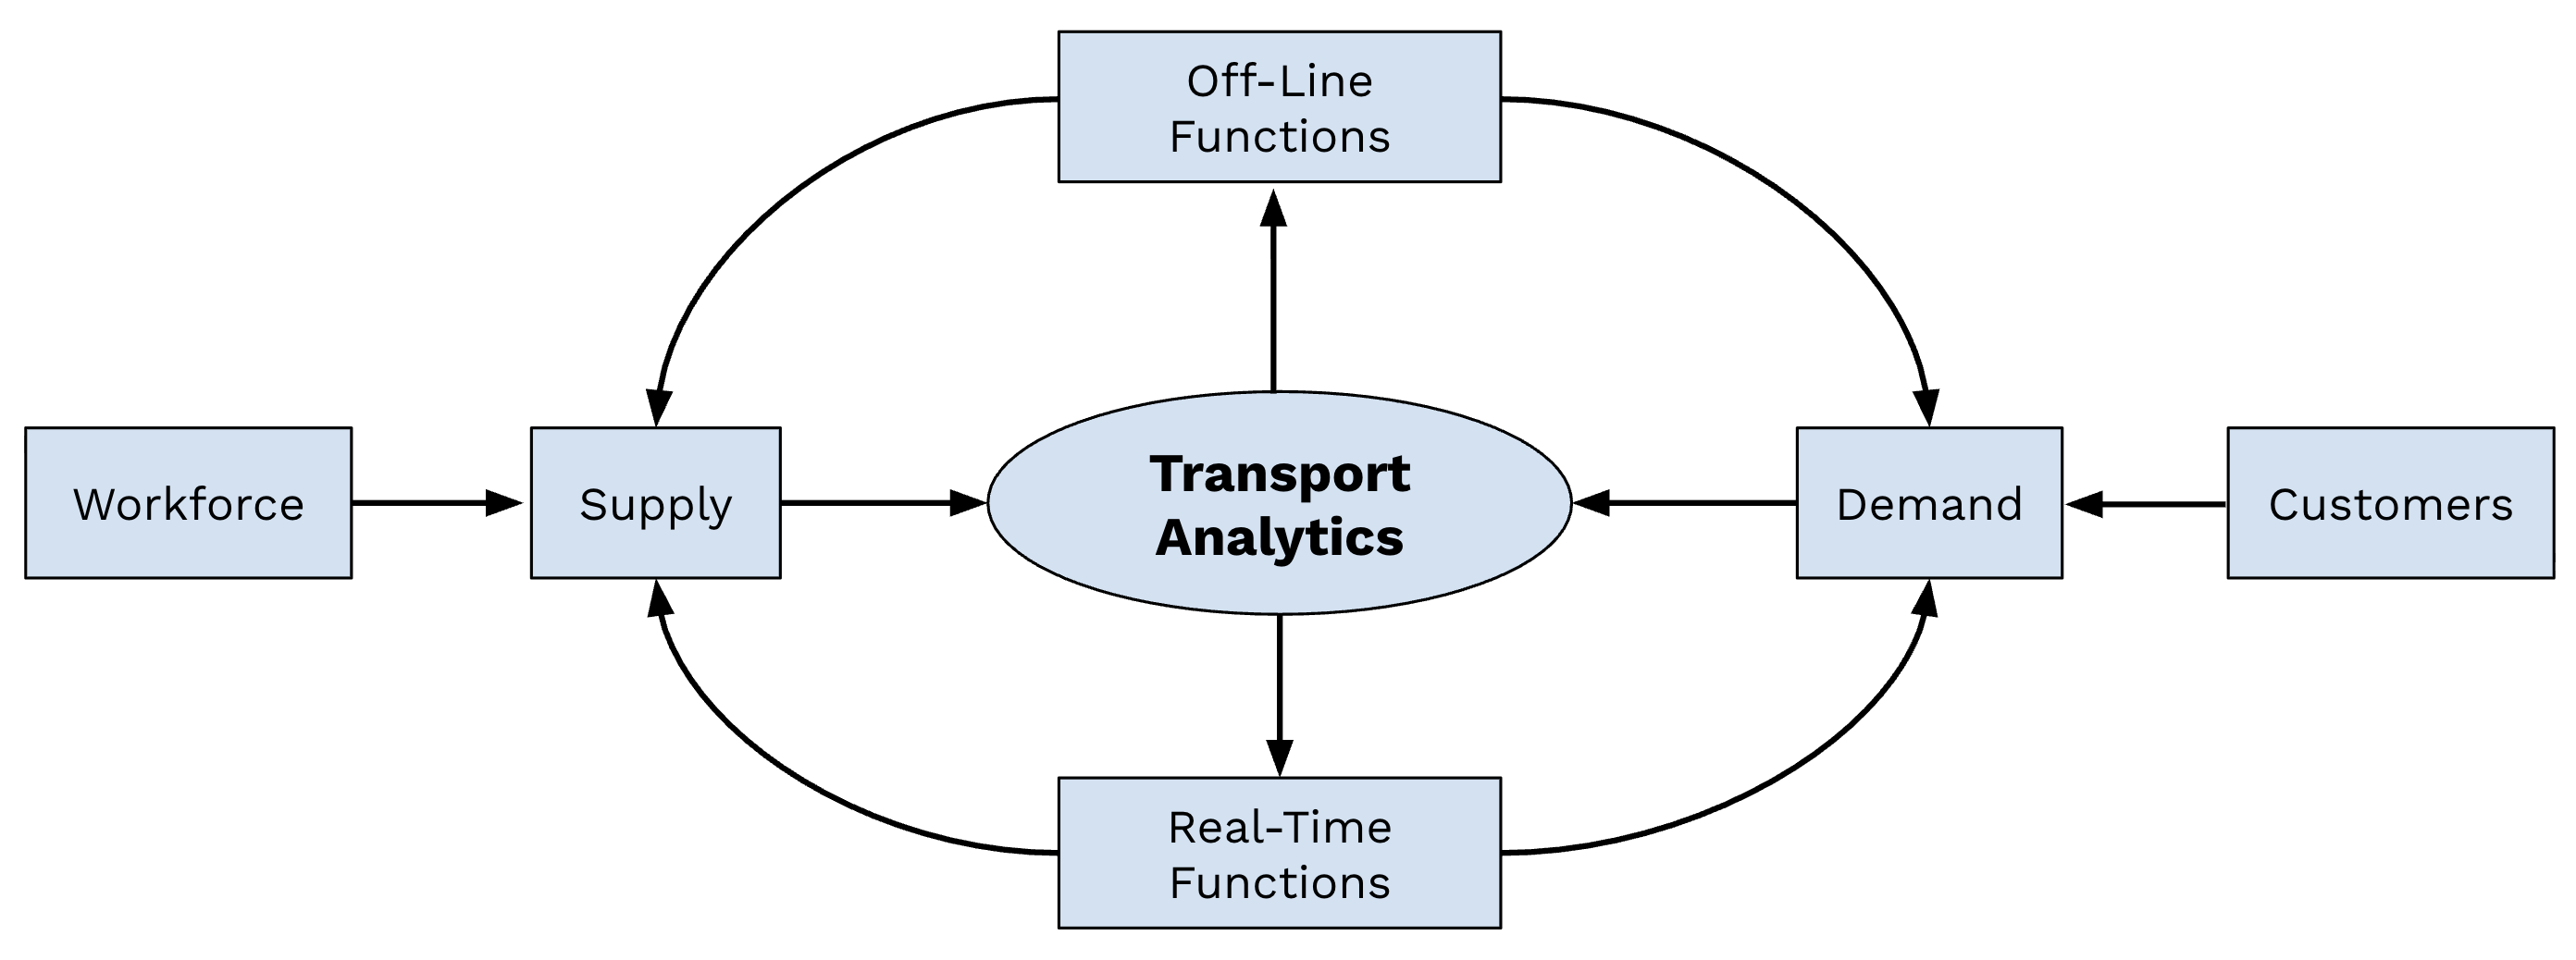
\includegraphics[width=\textwidth]{ai_graph.png}
\caption{AI Functions Framework}
\label{fig:ai}
\end{subfigure}
\caption{Reference frameworks from Professor Zhao's lecture}
\label{fig:frameworks}
\end{figure}

The framework illustrated in \autoref{fig:transport} shows how Transportation Analytics connects supply/demand through offline (planning) and real-time (operations) functions. Transport for London's evolution from manual surveys to smart cards to multimodal data fusion, as discussed in the lecture, demonstrates the shift toward predictive analytics.

Cities exist through multiple channels - numbers, graphs, images, language - and AI's power lies in unifying these data modalities.

\subsection*{Instructions:}
\begin{enumerate}[(a)]
\item \textbf{Adapt the Framework:} Using the transportation analytics framework as inspiration, create a similar diagram for your chosen domain from Exercise 1. Your framework should include:
\begin{itemize}
\item \textbf{Central Analytics Hub:} What would be equivalent to "Transport Analytics" in your domain?
\item \textbf{Supply Side:} What entities provide services/products/capabilities?
\item \textbf{Demand Side:} Who are the users/beneficiaries/customers?
\item \textbf{Offline Functions:} What long-term planning and strategic decisions occur?
\item \textbf{Real-time Functions:} What operational and tactical decisions happen in real-time?
\end{itemize}

\item \textbf{Data Flow Analysis:} Identify the key data sources and flows in your system:
\begin{itemize}
\item What data is generated by supply-side activities?
\item What data reflects demand-side behaviors?
\item How does this data feed into your central analytics function?
\item What are the feedback loops that enable optimization?
\end{itemize}

\item \textbf{AI Integration Opportunities:} Map AI's five core functions (represent, predict, explain, control, create) onto your framework:
\begin{itemize}
\item Where can AI \textit{represent} complex patterns in your domain?
\item How can \textit{prediction} capabilities improve outcomes?
\item Where is \textit{explanation} crucial for stakeholder trust?
\item What aspects of the system could benefit from AI \textit{control}?
\item How might \textit{generative} capabilities create new possibilities?
\end{itemize}
\end{enumerate}

\noindent\textbf{Goal:} Create a clear diagram (hand-drawn is fine) and reflect on your framework as if you would need to explain it to someone in your field. Include in your rationale, how it addresses the multi-channel nature of your domain (numbers, images, language, graphs). 

\section*{Exercise 3: Grounded AI Application}

Grounded AI is problem-driven (not technology-driven), context-aware, human-in-the-loop, deployment-ready, and iteratively co-created. It must be explainable to laypeople and address real needs within institutional and social constraints.

Examples include sentiment analysis (D.C. transit), crowd detection, bus dispatching optimization (Chicago), and workforce planning.

\subsection*{Instructions:}
\begin{enumerate}[(a)]
\item \textbf{Identify a Specific Problem:} Within your chosen domain, identify a concrete problem that could benefit from AI intervention. The problem should be:
\begin{itemize}
\item Clearly defined and bounded
\item Currently causing real pain points for stakeholders
\item Addressable through one or more of AI's five core functions
\item Amenable to human-AI collaboration
\end{itemize}

\item \textbf{Design a Grounded AI Solution:} Develop an AI application proposal that embodies grounded AI principles:
\begin{itemize}
\item \textbf{Problem-driven approach:} How does your solution address the real-world need?
\item \textbf{Context awareness:} What institutional, cultural, and social factors must be considered?
\item \textbf{Human-in-the-loop design:} How do humans maintain agency and oversight?
\item \textbf{Interpretability:} Can you explain your solution to a non-technical stakeholder?
\item \textbf{Iterative development:} How will you co-create and refine the solution with users?
\end{itemize}

\item \textbf{Implementation Considerations:} Address the practical aspects of deployment:
\begin{itemize}
\item What data would be required, and how would it be collected ethically?
\item What are the potential unintended consequences or failure modes?
\item How would you measure success and iterate based on feedback?
\item What stakeholder buy-in and change management would be necessary?
\end{itemize}

\item \textbf{Ethical and Social Impact:} Reflect on the broader implications:
\begin{itemize}
\item How does your solution advance equity and inclusion?
\item What privacy and consent considerations must be addressed?
\item How might your solution affect different stakeholder groups differently?
\end{itemize}
\end{enumerate}

\noindent\textbf{Goal:} Reflect on how a proposal for your grounded AI application could look like. Think of a structure that is brief and accessible for a non-technical decision-maker who needs to understand both the technical approach and its human implications.

\section*{Exercise 4: Communication and Reflection}

Effective communication translates complex AI concepts for diverse stakeholders. Professor Zhao demonstrated this through clear frameworks, compelling examples (Beijing comparison), and structured problem-solution thinking.

\subsection*{Instructions:}
\begin{enumerate}[(a)]
\item \textbf{Create a Stakeholder Communication Plan:} For your grounded AI application from Exercise 3, develop communication strategies for three different audiences:
\begin{itemize}
\item \textbf{Technical team:} How would you explain the AI approach, data requirements, and evaluation metrics?
\item \textbf{Community stakeholders:} How would you communicate benefits, address concerns, and gather input?
\item \textbf{Policymakers/executives:} How would you present the business case, risk mitigation, and strategic value?
\end{itemize}

\item \textbf{Anticipate and Address Concerns:} Identify potential objections or concerns each stakeholder group might have, and prepare thoughtful responses that demonstrate the grounded AI principles of transparency and human-centered design.

\item \textbf{Course Reflection:} Reflect on how this first lecture has shaped your understanding of AI in your chosen domain:
\begin{itemize}
\item What assumptions about technological progress did you reconsider?
\item How has the distinction between progress and success changed your perspective?
\item What questions do you now have about implementing AI responsibly in your field?
\item How do the concepts of behavioral thinking and computational thinking apply to your work?
\end{itemize}
\end{enumerate}

\noindent\textbf{Goal:} Reflect on how you can translate technical AI concepts into accessible language for diverse audiences.

\end{document}